\documentclass[twoside]{book}

% Packages required by doxygen
\usepackage{fixltx2e}
\usepackage{calc}
\usepackage{doxygen}
\usepackage[export]{adjustbox} % also loads graphicx
\usepackage{graphicx}
\usepackage[utf8]{inputenc}
\usepackage{makeidx}
\usepackage{multicol}
\usepackage{multirow}
\PassOptionsToPackage{warn}{textcomp}
\usepackage{textcomp}
\usepackage[nointegrals]{wasysym}
\usepackage[table]{xcolor}

% NLS support packages
\usepackage[spanish]{babel}
% Font selection
\usepackage[T1]{fontenc}
\usepackage[scaled=.90]{helvet}
\usepackage{courier}
\usepackage{amssymb}
\usepackage{sectsty}
\renewcommand{\familydefault}{\sfdefault}
\allsectionsfont{%
  \fontseries{bc}\selectfont%
  \color{darkgray}%
}
\renewcommand{\DoxyLabelFont}{%
  \fontseries{bc}\selectfont%
  \color{darkgray}%
}
\newcommand{\+}{\discretionary{\mbox{\scriptsize$\hookleftarrow$}}{}{}}

% Page & text layout
\usepackage{geometry}
\geometry{%
  a4paper,%
  top=2.5cm,%
  bottom=2.5cm,%
  left=2.5cm,%
  right=2.5cm%
}
\tolerance=750
\hfuzz=15pt
\hbadness=750
\setlength{\emergencystretch}{15pt}
\setlength{\parindent}{0cm}
\setlength{\parskip}{3ex plus 2ex minus 2ex}
\makeatletter
\renewcommand{\paragraph}{%
  \@startsection{paragraph}{4}{0ex}{-1.0ex}{1.0ex}{%
    \normalfont\normalsize\bfseries\SS@parafont%
  }%
}
\renewcommand{\subparagraph}{%
  \@startsection{subparagraph}{5}{0ex}{-1.0ex}{1.0ex}{%
    \normalfont\normalsize\bfseries\SS@subparafont%
  }%
}
\makeatother

% Headers & footers
\usepackage{fancyhdr}
\pagestyle{fancyplain}
\fancyhead[LE]{\fancyplain{}{\bfseries\thepage}}
\fancyhead[CE]{\fancyplain{}{}}
\fancyhead[RE]{\fancyplain{}{\bfseries\leftmark}}
\fancyhead[LO]{\fancyplain{}{\bfseries\rightmark}}
\fancyhead[CO]{\fancyplain{}{}}
\fancyhead[RO]{\fancyplain{}{\bfseries\thepage}}
\fancyfoot[LE]{\fancyplain{}{}}
\fancyfoot[CE]{\fancyplain{}{}}
\fancyfoot[RE]{\fancyplain{}{\bfseries\scriptsize Generado por Doxygen }}
\fancyfoot[LO]{\fancyplain{}{\bfseries\scriptsize Generado por Doxygen }}
\fancyfoot[CO]{\fancyplain{}{}}
\fancyfoot[RO]{\fancyplain{}{}}
\renewcommand{\footrulewidth}{0.4pt}
\renewcommand{\chaptermark}[1]{%
  \markboth{#1}{}%
}
\renewcommand{\sectionmark}[1]{%
  \markright{\thesection\ #1}%
}

% Indices & bibliography
\usepackage{natbib}
\usepackage[titles]{tocloft}
\setcounter{tocdepth}{3}
\setcounter{secnumdepth}{5}
\makeindex

% Hyperlinks (required, but should be loaded last)
\usepackage{ifpdf}
\ifpdf
  \usepackage[pdftex,pagebackref=true]{hyperref}
\else
  \usepackage[ps2pdf,pagebackref=true]{hyperref}
\fi
\hypersetup{%
  colorlinks=true,%
  linkcolor=blue,%
  citecolor=blue,%
  unicode%
}

% Custom commands
\newcommand{\clearemptydoublepage}{%
  \newpage{\pagestyle{empty}\cleardoublepage}%
}

\usepackage{caption}
\captionsetup{labelsep=space,justification=centering,font={bf},singlelinecheck=off,skip=4pt,position=top}

%===== C O N T E N T S =====

\begin{document}

% Titlepage & ToC
\hypersetup{pageanchor=false,
             bookmarksnumbered=true,
             pdfencoding=unicode
            }
\pagenumbering{roman}
\begin{titlepage}
\vspace*{7cm}
\begin{center}%
{\Large Círculo medio \\[1ex]\large 0 }\\
\vspace*{1cm}
{\large Generado por Doxygen 1.8.11}\\
\end{center}
\end{titlepage}
\clearemptydoublepage
\tableofcontents
\clearemptydoublepage
\pagenumbering{arabic}
\hypersetup{pageanchor=true}

%--- Begin generated contents ---
\chapter{Índice de clases}
\section{Lista de clases}
Lista de las clases, estructuras, uniones e interfaces con una breve descripción\+:\begin{DoxyCompactList}
\item\contentsline{section}{\hyperlink{classIntervalo}{Intervalo} }{\pageref{classIntervalo}}{}
\end{DoxyCompactList}

\chapter{Indice de archivos}
\section{Lista de archivos}
Lista de todos los archivos documentados y con descripciones breves\+:\begin{DoxyCompactList}
\item\contentsline{section}{\hyperlink{circulomedio_8cpp}{circulomedio.\+cpp} \\*Calcula círculo con centro en medio de dos círculos y radio la mitad de la distancia }{\pageref{circulomedio_8cpp}}{}
\end{DoxyCompactList}

\chapter{Documentación de las clases}
\hypertarget{classCirculo}{}\section{Referencia de la Clase Circulo}
\label{classCirculo}\index{Circulo@{Circulo}}


Clase Círculo.  


\subsection*{Métodos públicos}
\begin{DoxyCompactItemize}
\item 
\hyperlink{classCirculo_a6933bf908b78a4167684081a3a8f257f}{Circulo} ()\hypertarget{classCirculo_a6933bf908b78a4167684081a3a8f257f}{}\label{classCirculo_a6933bf908b78a4167684081a3a8f257f}

\begin{DoxyCompactList}\small\item\em Constructor\+: Pone a 0 el punto y el radio. \end{DoxyCompactList}\item 
\hyperlink{classCirculo_ad4c6c76f0227c25afcb872a8744ebe56}{Circulo} (\hyperlink{classPunto}{Punto} centro, double radio)\hypertarget{classCirculo_ad4c6c76f0227c25afcb872a8744ebe56}{}\label{classCirculo_ad4c6c76f0227c25afcb872a8744ebe56}

\begin{DoxyCompactList}\small\item\em Constructor\+: Inicializa el círculo con un centro y un radio. \end{DoxyCompactList}\item 
void \hyperlink{classCirculo_aa24cc4b316a3d9ece35f120d9b8e1fc4}{set} (\hyperlink{classPunto}{Punto} centro, double radio)\hypertarget{classCirculo_aa24cc4b316a3d9ece35f120d9b8e1fc4}{}\label{classCirculo_aa24cc4b316a3d9ece35f120d9b8e1fc4}

\begin{DoxyCompactList}\small\item\em Asigna el centro y el radio a un circulo. \end{DoxyCompactList}\item 
\hyperlink{classPunto}{Punto} \hyperlink{classCirculo_a022cde4d10d14a47a3b3921f80909f3b}{get\+Centro} () const \hypertarget{classCirculo_a022cde4d10d14a47a3b3921f80909f3b}{}\label{classCirculo_a022cde4d10d14a47a3b3921f80909f3b}

\begin{DoxyCompactList}\small\item\em Devuelve el centro de un circulo. \end{DoxyCompactList}\item 
double \hyperlink{classCirculo_a982f8a785d8a68ab1483b609cd752980}{get\+Radio} () const \hypertarget{classCirculo_a982f8a785d8a68ab1483b609cd752980}{}\label{classCirculo_a982f8a785d8a68ab1483b609cd752980}

\begin{DoxyCompactList}\small\item\em Devuelve el radio de un circulo. \end{DoxyCompactList}\item 
void \hyperlink{classCirculo_a2deaed49ea394702beb0554f9480137e}{escribir} () const \hypertarget{classCirculo_a2deaed49ea394702beb0554f9480137e}{}\label{classCirculo_a2deaed49ea394702beb0554f9480137e}

\begin{DoxyCompactList}\small\item\em Escribe círculo en formato radio-\/centro. \end{DoxyCompactList}\item 
void \hyperlink{classCirculo_aa71efffb3b42eeaefd43743a8d34aa74}{leer} ()\hypertarget{classCirculo_aa71efffb3b42eeaefd43743a8d34aa74}{}\label{classCirculo_aa71efffb3b42eeaefd43743a8d34aa74}

\begin{DoxyCompactList}\small\item\em lee círculo en formato radio-\/centro \end{DoxyCompactList}\item 
double \hyperlink{classCirculo_a532d4f2bd03b688403c4370319411dc3}{area} () const \hypertarget{classCirculo_a532d4f2bd03b688403c4370319411dc3}{}\label{classCirculo_a532d4f2bd03b688403c4370319411dc3}

\begin{DoxyCompactList}\small\item\em Devuelve el área de un círculo. \end{DoxyCompactList}\end{DoxyCompactItemize}


\subsection{Descripción detallada}
Clase Círculo. 

Definición en la línea 85 del archivo circulomedio.\+cpp.



La documentación para esta clase fue generada a partir del siguiente fichero\+:\begin{DoxyCompactItemize}
\item 
\hyperlink{circulomedio_8cpp}{circulomedio.\+cpp}\end{DoxyCompactItemize}

\hypertarget{classPunto}{}\section{Referencia de la Clase Punto}
\label{classPunto}\index{Punto@{Punto}}


Clase \hyperlink{classPunto}{Punto}.  


\subsection*{Métodos públicos}
\begin{DoxyCompactItemize}
\item 
\hyperlink{classPunto_a4b8b70b933ff13493ee5ddb3c8532c10}{Punto} ()\hypertarget{classPunto_a4b8b70b933ff13493ee5ddb3c8532c10}{}\label{classPunto_a4b8b70b933ff13493ee5ddb3c8532c10}

\begin{DoxyCompactList}\small\item\em constructor. Pone a 0 las dos coordenadas \end{DoxyCompactList}\item 
\hyperlink{classPunto_a911bb8d88eaa1f9904a27b0e159a51c0}{Punto} (double x, double y)\hypertarget{classPunto_a911bb8d88eaa1f9904a27b0e159a51c0}{}\label{classPunto_a911bb8d88eaa1f9904a27b0e159a51c0}

\begin{DoxyCompactList}\small\item\em constructor. Inicializa un punto con dos valores x y \end{DoxyCompactList}\item 
double \hyperlink{classPunto_aa218292fec9bad5ec6d71d4bd9173d9d}{getX} () const \hypertarget{classPunto_aa218292fec9bad5ec6d71d4bd9173d9d}{}\label{classPunto_aa218292fec9bad5ec6d71d4bd9173d9d}

\begin{DoxyCompactList}\small\item\em Devuelve la coordenada x del punto. \end{DoxyCompactList}\item 
double \hyperlink{classPunto_a214978b8bbae48ca5927f2e56fb3bd22}{getY} () const \hypertarget{classPunto_a214978b8bbae48ca5927f2e56fb3bd22}{}\label{classPunto_a214978b8bbae48ca5927f2e56fb3bd22}

\begin{DoxyCompactList}\small\item\em Devuelve la coordenada y del punto. \end{DoxyCompactList}\item 
void \hyperlink{classPunto_a51ae6616f828bb2b4111bc8ace49dbca}{setX} (double nuevoX)\hypertarget{classPunto_a51ae6616f828bb2b4111bc8ace49dbca}{}\label{classPunto_a51ae6616f828bb2b4111bc8ace49dbca}

\begin{DoxyCompactList}\small\item\em Asigna el valor nuevoX a la coordenada x del punto. \end{DoxyCompactList}\item 
void \hyperlink{classPunto_a6a0f8adb5946f31a7867a06f54d97462}{setY} (double nuevoY)\hypertarget{classPunto_a6a0f8adb5946f31a7867a06f54d97462}{}\label{classPunto_a6a0f8adb5946f31a7867a06f54d97462}

\begin{DoxyCompactList}\small\item\em Asigna el valor nuevoY a la coordenada y del punto. \end{DoxyCompactList}\item 
void \hyperlink{classPunto_afc543b48134f632fa354d8b027954e80}{escribir} () const \hypertarget{classPunto_afc543b48134f632fa354d8b027954e80}{}\label{classPunto_afc543b48134f632fa354d8b027954e80}

\begin{DoxyCompactList}\small\item\em Escribe un punto en formato (x,y) \end{DoxyCompactList}\item 
void \hyperlink{classPunto_a84cc9b0ee2e5b00842e7bff819b80459}{leer} ()\hypertarget{classPunto_a84cc9b0ee2e5b00842e7bff819b80459}{}\label{classPunto_a84cc9b0ee2e5b00842e7bff819b80459}

\begin{DoxyCompactList}\small\item\em // Lee un punto en el formato (x,y) \end{DoxyCompactList}\end{DoxyCompactItemize}


\subsection{Descripción detallada}
Clase \hyperlink{classPunto}{Punto}. 

Definición en la línea 18 del archivo circulomedio.\+cpp.



La documentación para esta clase fue generada a partir del siguiente fichero\+:\begin{DoxyCompactItemize}
\item 
\hyperlink{circulomedio_8cpp}{circulomedio.\+cpp}\end{DoxyCompactItemize}

\chapter{Documentación de archivos}
\hypertarget{circulo_8h}{}\section{Referencia del Archivo include/circulo.h}
\label{circulo_8h}\index{include/circulo.\+h@{include/circulo.\+h}}


Definición de la clase {\ttfamily \hyperlink{classCirculo}{Circulo}}.  


{\ttfamily \#include \char`\"{}punto.\+h\char`\"{}}\\*
Dependencia gráfica adjunta para circulo.\+h\+:
\nopagebreak
\begin{figure}[H]
\begin{center}
\leavevmode
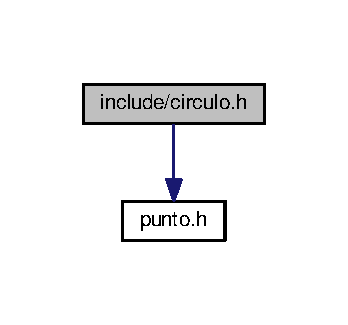
\includegraphics[width=167pt]{circulo_8h__incl}
\end{center}
\end{figure}
Gráfico de los archivos que directa o indirectamente incluyen a este archivo\+:
\nopagebreak
\begin{figure}[H]
\begin{center}
\leavevmode
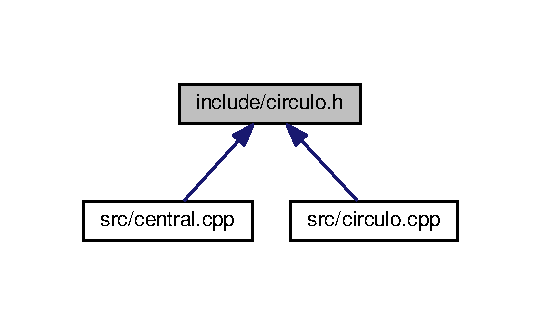
\includegraphics[width=260pt]{circulo_8h__dep__incl}
\end{center}
\end{figure}
\subsection*{Clases}
\begin{DoxyCompactItemize}
\item 
class \hyperlink{classCirculo}{Circulo}
\end{DoxyCompactItemize}
\subsection*{Funciones}
\begin{DoxyCompactItemize}
\item 
double \hyperlink{circulo_8h_a2be093c30676e02d6f76b6a56c713b34}{distancia} (\hyperlink{classCirculo}{Circulo} c1, \hyperlink{classCirculo}{Circulo} c2)
\begin{DoxyCompactList}\small\item\em Calcula la distancia entre dos circulos. \end{DoxyCompactList}\item 
bool \hyperlink{circulo_8h_a6e60e1271c0a8f48e87f8e53b434dfd4}{interior} (\hyperlink{classPunto}{Punto} p, \hyperlink{classCirculo}{Circulo} c)
\begin{DoxyCompactList}\small\item\em Comprueba si un punto es interior a un círculo. \end{DoxyCompactList}\end{DoxyCompactItemize}


\subsection{Descripción detallada}
Definición de la clase {\ttfamily \hyperlink{classCirculo}{Circulo}}. 

\begin{DoxyAuthor}{Autor}
M\+P-\/\+D\+G\+IM -\/ Grupo A 
\end{DoxyAuthor}


\subsection{Documentación de las funciones}
\index{circulo.\+h@{circulo.\+h}!distancia@{distancia}}
\index{distancia@{distancia}!circulo.\+h@{circulo.\+h}}
\subsubsection[{\texorpdfstring{distancia(\+Circulo c1, Circulo c2)}{distancia(Circulo c1, Circulo c2)}}]{\setlength{\rightskip}{0pt plus 5cm}double distancia (
\begin{DoxyParamCaption}
\item[{{\bf Circulo}}]{c1, }
\item[{{\bf Circulo}}]{c2}
\end{DoxyParamCaption}
)}\hypertarget{circulo_8h_a2be093c30676e02d6f76b6a56c713b34}{}\label{circulo_8h_a2be093c30676e02d6f76b6a56c713b34}


Calcula la distancia entre dos circulos. 


\begin{DoxyParams}{Parámetros}
{\em c1} & primer círculo \\
\hline
{\em c2} & segundo círculo \\
\hline
\end{DoxyParams}
\begin{DoxyReturn}{Devuelve}
la distancia entre el círculo {\itshape c1} y el círculo {\itshape c2} 
\end{DoxyReturn}
La distancia entre dos círculos se define como la distancia entre los centros menos los dos radios. Nótese que la distancia puede ser negativa si los círculos se intersecan 

Definición en la línea 65 del archivo circulo.\+cpp.


\begin{DoxyCode}
65                                          \{
66     \hyperlink{classPunto}{Punto} centro1, centro2;
67     \textcolor{keywordtype}{double} dist;
68 
69     centro1=c1.\hyperlink{classCirculo_a022cde4d10d14a47a3b3921f80909f3b}{getCentro}();
70     centro2=c2.\hyperlink{classCirculo_a022cde4d10d14a47a3b3921f80909f3b}{getCentro}();
71     dist=\hyperlink{circulo_8cpp_a2be093c30676e02d6f76b6a56c713b34}{distancia}(centro1,centro2)-c1.\hyperlink{classCirculo_a982f8a785d8a68ab1483b609cd752980}{getRadio}()-c2.\hyperlink{classCirculo_a982f8a785d8a68ab1483b609cd752980}{getRadio}();
72     \textcolor{keywordflow}{return} dist;
73 \}
\end{DoxyCode}


Gráfico de llamadas para esta función\+:
\nopagebreak
\begin{figure}[H]
\begin{center}
\leavevmode
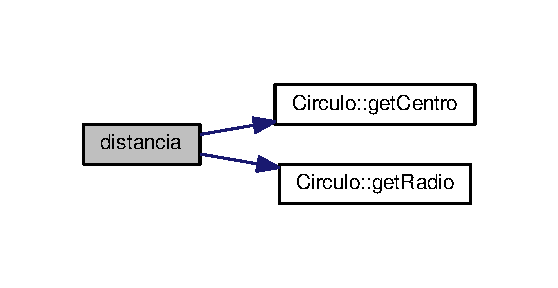
\includegraphics[width=268pt]{circulo_8h_a2be093c30676e02d6f76b6a56c713b34_cgraph}
\end{center}
\end{figure}


\index{circulo.\+h@{circulo.\+h}!interior@{interior}}
\index{interior@{interior}!circulo.\+h@{circulo.\+h}}
\subsubsection[{\texorpdfstring{interior(\+Punto p, Circulo c)}{interior(Punto p, Circulo c)}}]{\setlength{\rightskip}{0pt plus 5cm}bool interior (
\begin{DoxyParamCaption}
\item[{{\bf Punto}}]{p, }
\item[{{\bf Circulo}}]{c}
\end{DoxyParamCaption}
)}\hypertarget{circulo_8h_a6e60e1271c0a8f48e87f8e53b434dfd4}{}\label{circulo_8h_a6e60e1271c0a8f48e87f8e53b434dfd4}


Comprueba si un punto es interior a un círculo. 


\begin{DoxyParams}{Parámetros}
{\em p} & punto a comprobar \\
\hline
{\em c} & circulo \\
\hline
\end{DoxyParams}

\begin{DoxyRetVals}{Valores devueltos}
{\em true} & si el punto {\itshape p} es interior al círculo {\itshape c} \\
\hline
{\em false} & en caso contrario \\
\hline
\end{DoxyRetVals}


Definición en la línea 83 del archivo circulo.\+cpp.


\begin{DoxyCode}
83                                   \{
84     \textcolor{keywordflow}{if}(\hyperlink{circulo_8cpp_a2be093c30676e02d6f76b6a56c713b34}{distancia}(p,c.\hyperlink{classCirculo_a022cde4d10d14a47a3b3921f80909f3b}{getCentro}())<=c.\hyperlink{classCirculo_a982f8a785d8a68ab1483b609cd752980}{getRadio}()) \{
85         \textcolor{keywordflow}{return} \textcolor{keyword}{true};
86     \}
87     \textcolor{keywordflow}{else}\{
88         \textcolor{keywordflow}{return} \textcolor{keyword}{false};
89     \}
90 \}
\end{DoxyCode}


Gráfico de llamadas para esta función\+:
\nopagebreak
\begin{figure}[H]
\begin{center}
\leavevmode
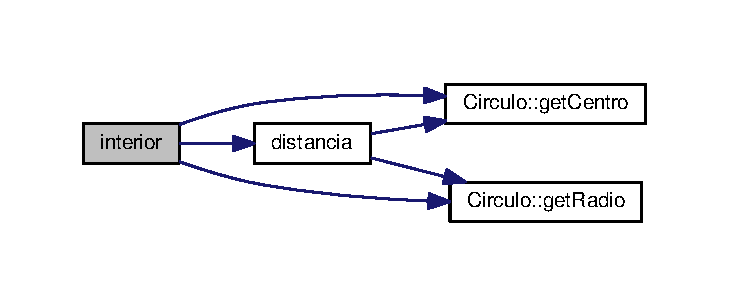
\includegraphics[width=350pt]{circulo_8h_a6e60e1271c0a8f48e87f8e53b434dfd4_cgraph}
\end{center}
\end{figure}



\hypertarget{punto_8h}{}\section{Referencia del Archivo include/punto.h}
\label{punto_8h}\index{include/punto.\+h@{include/punto.\+h}}


Definción de la clase {\ttfamily \hyperlink{classPunto}{Punto}}.  


Gráfico de los archivos que directa o indirectamente incluyen a este archivo\+:
\nopagebreak
\begin{figure}[H]
\begin{center}
\leavevmode
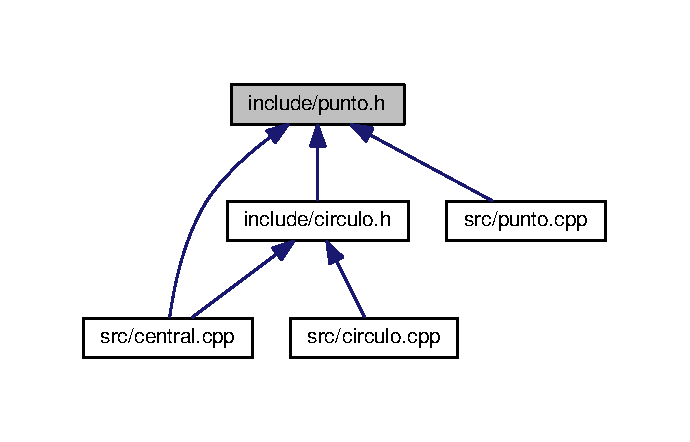
\includegraphics[width=331pt]{punto_8h__dep__incl}
\end{center}
\end{figure}
\subsection*{Clases}
\begin{DoxyCompactItemize}
\item 
class \hyperlink{classPunto}{Punto}
\begin{DoxyCompactList}\small\item\em Clase \hyperlink{classPunto}{Punto}. \end{DoxyCompactList}\end{DoxyCompactItemize}
\subsection*{Funciones}
\begin{DoxyCompactItemize}
\item 
double \hyperlink{punto_8h_a9c93fd6721d3b594dbbcfb77a92a2880}{distancia} (\hyperlink{classPunto}{Punto} p1, \hyperlink{classPunto}{Punto} p2)
\begin{DoxyCompactList}\small\item\em Funciones auxiliares (no son métodos de la clase) \end{DoxyCompactList}\item 
\hyperlink{classPunto}{Punto} \hyperlink{punto_8h_a119f914f219e98be4c2c93b5138e97da}{punto\+Medio} (\hyperlink{classPunto}{Punto} p1, \hyperlink{classPunto}{Punto} p2)
\begin{DoxyCompactList}\small\item\em Calcula el punto que está entre dos puntos dados con distancia mínima a ambos. \end{DoxyCompactList}\end{DoxyCompactItemize}


\subsection{Descripción detallada}
Definción de la clase {\ttfamily \hyperlink{classPunto}{Punto}}. 

\begin{DoxyAuthor}{Autor}
M\+P-\/\+D\+G\+IM -\/ Grupo A 
\end{DoxyAuthor}


\subsection{Documentación de las funciones}
\index{punto.\+h@{punto.\+h}!distancia@{distancia}}
\index{distancia@{distancia}!punto.\+h@{punto.\+h}}
\subsubsection[{\texorpdfstring{distancia(\+Punto p1, Punto p2)}{distancia(Punto p1, Punto p2)}}]{\setlength{\rightskip}{0pt plus 5cm}double distancia (
\begin{DoxyParamCaption}
\item[{{\bf Punto}}]{p1, }
\item[{{\bf Punto}}]{p2}
\end{DoxyParamCaption}
)}\hypertarget{punto_8h_a9c93fd6721d3b594dbbcfb77a92a2880}{}\label{punto_8h_a9c93fd6721d3b594dbbcfb77a92a2880}


Funciones auxiliares (no son métodos de la clase) 

Calcula la distancia entre dos puntos 
\begin{DoxyParams}{Parámetros}
{\em p1} & primer punto \\
\hline
{\em p2} & segundo punto \\
\hline
\end{DoxyParams}
\begin{DoxyReturn}{Devuelve}
la distancia entre el punto {\itshape p1} y el punto {\itshape p2} 
\end{DoxyReturn}


Definición en la línea 40 del archivo punto.\+cpp.


\begin{DoxyCode}
40                                     \{
41     \textcolor{keywordflow}{return} sqrt((p1.\hyperlink{classPunto_aa218292fec9bad5ec6d71d4bd9173d9d}{getX}()-p2.\hyperlink{classPunto_aa218292fec9bad5ec6d71d4bd9173d9d}{getX}())*(p1.\hyperlink{classPunto_aa218292fec9bad5ec6d71d4bd9173d9d}{getX}()-p2.\hyperlink{classPunto_aa218292fec9bad5ec6d71d4bd9173d9d}{getX}()) +
42          (p1.\hyperlink{classPunto_a214978b8bbae48ca5927f2e56fb3bd22}{getY}()-p2.\hyperlink{classPunto_a214978b8bbae48ca5927f2e56fb3bd22}{getY}())*(p1.\hyperlink{classPunto_a214978b8bbae48ca5927f2e56fb3bd22}{getY}()-p2.\hyperlink{classPunto_a214978b8bbae48ca5927f2e56fb3bd22}{getY}()));
43 \}
\end{DoxyCode}


Gráfico de llamadas para esta función\+:
\nopagebreak
\begin{figure}[H]
\begin{center}
\leavevmode
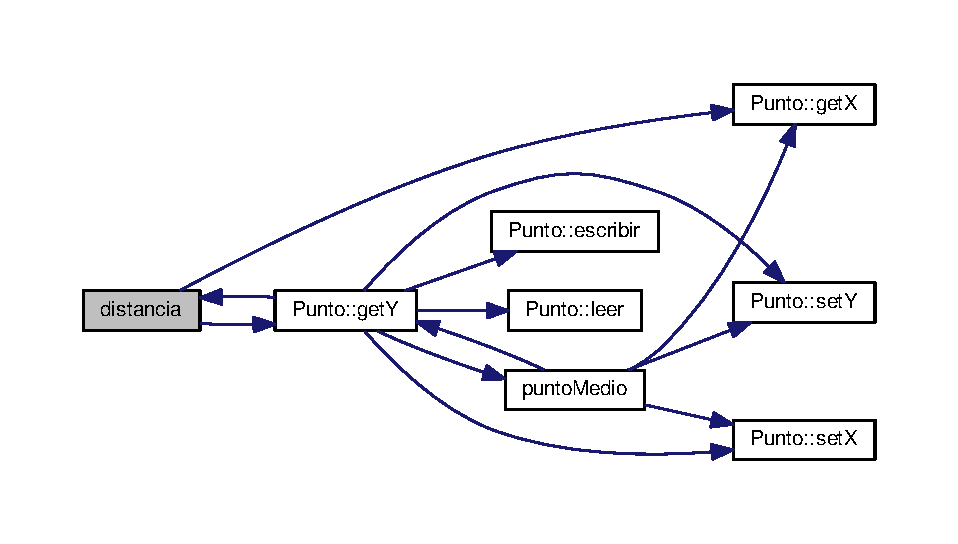
\includegraphics[width=350pt]{punto_8h_a9c93fd6721d3b594dbbcfb77a92a2880_cgraph}
\end{center}
\end{figure}


\index{punto.\+h@{punto.\+h}!punto\+Medio@{punto\+Medio}}
\index{punto\+Medio@{punto\+Medio}!punto.\+h@{punto.\+h}}
\subsubsection[{\texorpdfstring{punto\+Medio(\+Punto p1, Punto p2)}{puntoMedio(Punto p1, Punto p2)}}]{\setlength{\rightskip}{0pt plus 5cm}{\bf Punto} punto\+Medio (
\begin{DoxyParamCaption}
\item[{{\bf Punto}}]{p1, }
\item[{{\bf Punto}}]{p2}
\end{DoxyParamCaption}
)}\hypertarget{punto_8h_a119f914f219e98be4c2c93b5138e97da}{}\label{punto_8h_a119f914f219e98be4c2c93b5138e97da}


Calcula el punto que está entre dos puntos dados con distancia mínima a ambos. 


\begin{DoxyParams}{Parámetros}
{\em p1} & primer punto \\
\hline
{\em p2} & segundo punto \\
\hline
\end{DoxyParams}
\begin{DoxyReturn}{Devuelve}
un punto entre el punto {\itshape p1} y el punto {\itshape p2} con distancia mínima a ambos 
\end{DoxyReturn}


Definición en la línea 53 del archivo punto.\+cpp.


\begin{DoxyCode}
53                                     \{
54     \hyperlink{classPunto}{Punto} pMedio;
55     pMedio.\hyperlink{classPunto_a51ae6616f828bb2b4111bc8ace49dbca}{setX}((p1.\hyperlink{classPunto_aa218292fec9bad5ec6d71d4bd9173d9d}{getX}()+p2.\hyperlink{classPunto_aa218292fec9bad5ec6d71d4bd9173d9d}{getX}())/2.0);
56     pMedio.\hyperlink{classPunto_a6a0f8adb5946f31a7867a06f54d97462}{setY}((p1.\hyperlink{classPunto_a214978b8bbae48ca5927f2e56fb3bd22}{getY}()+p2.\hyperlink{classPunto_a214978b8bbae48ca5927f2e56fb3bd22}{getY}())/2.0);
57     \textcolor{keywordflow}{return} pMedio;
58 \}
\end{DoxyCode}


Gráfico de llamadas para esta función\+:
\nopagebreak
\begin{figure}[H]
\begin{center}
\leavevmode
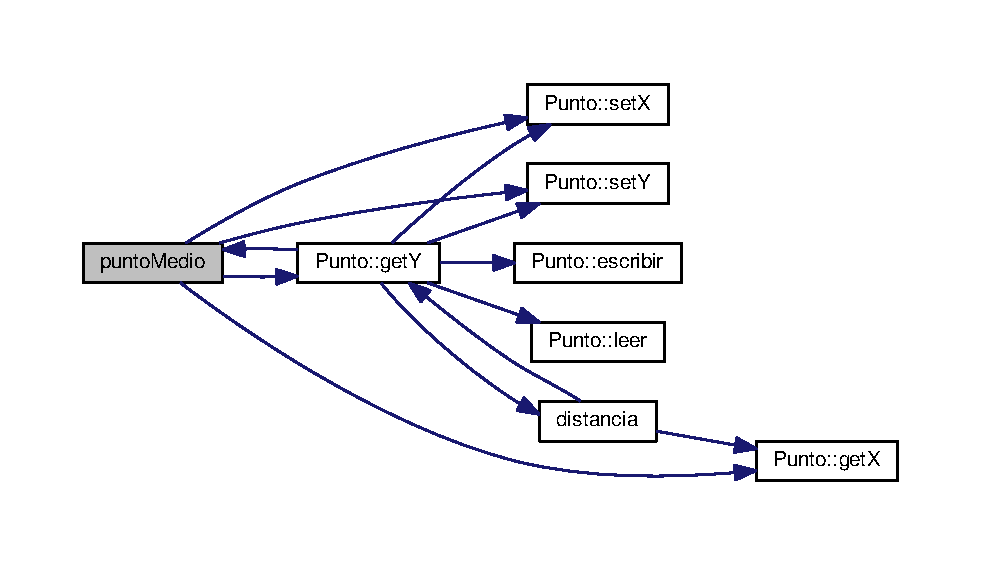
\includegraphics[width=350pt]{punto_8h_a119f914f219e98be4c2c93b5138e97da_cgraph}
\end{center}
\end{figure}



\hypertarget{central_8cpp}{}\section{Referencia del Archivo src/central.cpp}
\label{central_8cpp}\index{src/central.\+cpp@{src/central.\+cpp}}


Implementación del programa principal.  


{\ttfamily \#include $<$iostream$>$}\\*
{\ttfamily \#include \char`\"{}punto.\+h\char`\"{}}\\*
{\ttfamily \#include \char`\"{}circulo.\+h\char`\"{}}\\*
Dependencia gráfica adjunta para central.\+cpp\+:
\nopagebreak
\begin{figure}[H]
\begin{center}
\leavevmode
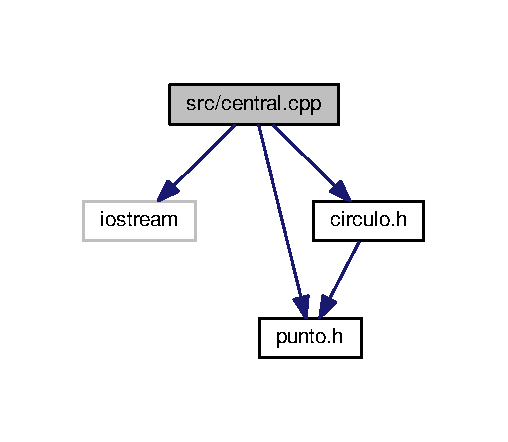
\includegraphics[width=244pt]{central_8cpp__incl}
\end{center}
\end{figure}
\subsection*{Funciones}
\begin{DoxyCompactItemize}
\item 
int {\bfseries main} ()\hypertarget{central_8cpp_ae66f6b31b5ad750f1fe042a706a4e3d4}{}\label{central_8cpp_ae66f6b31b5ad750f1fe042a706a4e3d4}

\end{DoxyCompactItemize}


\subsection{Descripción detallada}
Implementación del programa principal. 

\begin{DoxyAuthor}{Autor}
M\+P-\/\+D\+G\+IM -\/ Grupo A 
\end{DoxyAuthor}

\hypertarget{circulo_8cpp}{}\section{Referencia del Archivo src/circulo.cpp}
\label{circulo_8cpp}\index{src/circulo.\+cpp@{src/circulo.\+cpp}}


Implementación de la clase {\ttfamily \hyperlink{classCirculo}{Circulo}}.  


{\ttfamily \#include $<$iostream$>$}\\*
{\ttfamily \#include $<$cmath$>$}\\*
{\ttfamily \#include \char`\"{}circulo.\+h\char`\"{}}\\*
Dependencia gráfica adjunta para circulo.\+cpp\+:
\nopagebreak
\begin{figure}[H]
\begin{center}
\leavevmode
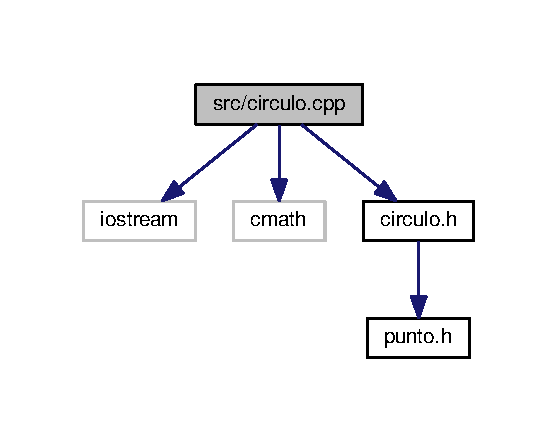
\includegraphics[width=268pt]{circulo_8cpp__incl}
\end{center}
\end{figure}
\subsection*{Funciones}
\begin{DoxyCompactItemize}
\item 
double \hyperlink{circulo_8cpp_a2be093c30676e02d6f76b6a56c713b34}{distancia} (\hyperlink{classCirculo}{Circulo} c1, \hyperlink{classCirculo}{Circulo} c2)
\begin{DoxyCompactList}\small\item\em Calcula la distancia entre dos circulos. \end{DoxyCompactList}\item 
bool \hyperlink{circulo_8cpp_a6e60e1271c0a8f48e87f8e53b434dfd4}{interior} (\hyperlink{classPunto}{Punto} p, \hyperlink{classCirculo}{Circulo} c)
\begin{DoxyCompactList}\small\item\em Comprueba si un punto es interior a un círculo. \end{DoxyCompactList}\end{DoxyCompactItemize}


\subsection{Descripción detallada}
Implementación de la clase {\ttfamily \hyperlink{classCirculo}{Circulo}}. 

\begin{DoxyAuthor}{Autor}
M\+P-\/\+D\+G\+IM -\/ Grupo A 
\end{DoxyAuthor}


\subsection{Documentación de las funciones}
\index{circulo.\+cpp@{circulo.\+cpp}!distancia@{distancia}}
\index{distancia@{distancia}!circulo.\+cpp@{circulo.\+cpp}}
\subsubsection[{\texorpdfstring{distancia(\+Circulo c1, Circulo c2)}{distancia(Circulo c1, Circulo c2)}}]{\setlength{\rightskip}{0pt plus 5cm}double distancia (
\begin{DoxyParamCaption}
\item[{{\bf Circulo}}]{c1, }
\item[{{\bf Circulo}}]{c2}
\end{DoxyParamCaption}
)}\hypertarget{circulo_8cpp_a2be093c30676e02d6f76b6a56c713b34}{}\label{circulo_8cpp_a2be093c30676e02d6f76b6a56c713b34}


Calcula la distancia entre dos circulos. 


\begin{DoxyParams}{Parámetros}
{\em c1} & primer círculo \\
\hline
{\em c2} & segundo círculo \\
\hline
\end{DoxyParams}
\begin{DoxyReturn}{Devuelve}
la distancia entre el círculo {\itshape c1} y el círculo {\itshape c2} 
\end{DoxyReturn}
La distancia entre dos círculos se define como la distancia entre los centros menos los dos radios. Nótese que la distancia puede ser negativa si los círculos se intersecan 

Definición en la línea 65 del archivo circulo.\+cpp.


\begin{DoxyCode}
65                                          \{
66     \hyperlink{classPunto}{Punto} centro1, centro2;
67     \textcolor{keywordtype}{double} dist;
68 
69     centro1=c1.\hyperlink{classCirculo_a022cde4d10d14a47a3b3921f80909f3b}{getCentro}();
70     centro2=c2.\hyperlink{classCirculo_a022cde4d10d14a47a3b3921f80909f3b}{getCentro}();
71     dist=\hyperlink{circulo_8cpp_a2be093c30676e02d6f76b6a56c713b34}{distancia}(centro1,centro2)-c1.\hyperlink{classCirculo_a982f8a785d8a68ab1483b609cd752980}{getRadio}()-c2.\hyperlink{classCirculo_a982f8a785d8a68ab1483b609cd752980}{getRadio}();
72     \textcolor{keywordflow}{return} dist;
73 \}
\end{DoxyCode}


Gráfico de llamadas para esta función\+:
\nopagebreak
\begin{figure}[H]
\begin{center}
\leavevmode
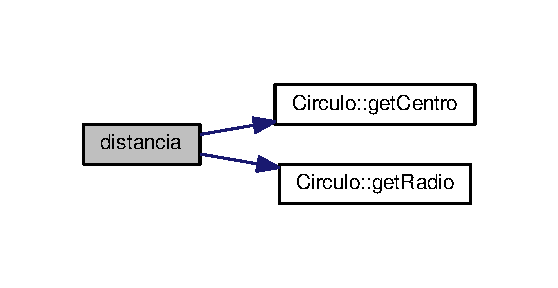
\includegraphics[width=268pt]{circulo_8cpp_a2be093c30676e02d6f76b6a56c713b34_cgraph}
\end{center}
\end{figure}


\index{circulo.\+cpp@{circulo.\+cpp}!interior@{interior}}
\index{interior@{interior}!circulo.\+cpp@{circulo.\+cpp}}
\subsubsection[{\texorpdfstring{interior(\+Punto p, Circulo c)}{interior(Punto p, Circulo c)}}]{\setlength{\rightskip}{0pt plus 5cm}bool interior (
\begin{DoxyParamCaption}
\item[{{\bf Punto}}]{p, }
\item[{{\bf Circulo}}]{c}
\end{DoxyParamCaption}
)}\hypertarget{circulo_8cpp_a6e60e1271c0a8f48e87f8e53b434dfd4}{}\label{circulo_8cpp_a6e60e1271c0a8f48e87f8e53b434dfd4}


Comprueba si un punto es interior a un círculo. 


\begin{DoxyParams}{Parámetros}
{\em p} & punto a comprobar \\
\hline
{\em c} & circulo \\
\hline
\end{DoxyParams}

\begin{DoxyRetVals}{Valores devueltos}
{\em true} & si el punto {\itshape p} es interior al círculo {\itshape c} \\
\hline
{\em false} & en caso contrario \\
\hline
\end{DoxyRetVals}


Definición en la línea 83 del archivo circulo.\+cpp.


\begin{DoxyCode}
83                                   \{
84     \textcolor{keywordflow}{if}(\hyperlink{circulo_8cpp_a2be093c30676e02d6f76b6a56c713b34}{distancia}(p,c.\hyperlink{classCirculo_a022cde4d10d14a47a3b3921f80909f3b}{getCentro}())<=c.\hyperlink{classCirculo_a982f8a785d8a68ab1483b609cd752980}{getRadio}()) \{
85         \textcolor{keywordflow}{return} \textcolor{keyword}{true};
86     \}
87     \textcolor{keywordflow}{else}\{
88         \textcolor{keywordflow}{return} \textcolor{keyword}{false};
89     \}
90 \}
\end{DoxyCode}


Gráfico de llamadas para esta función\+:
\nopagebreak
\begin{figure}[H]
\begin{center}
\leavevmode
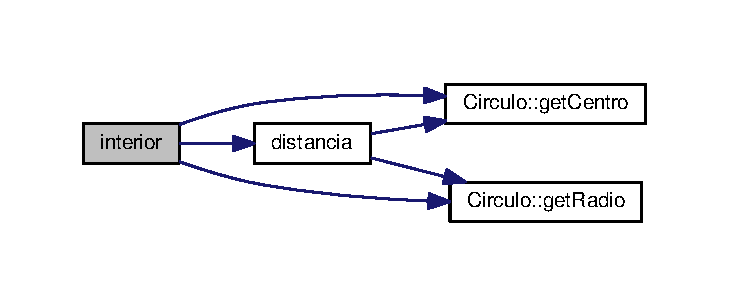
\includegraphics[width=350pt]{circulo_8cpp_a6e60e1271c0a8f48e87f8e53b434dfd4_cgraph}
\end{center}
\end{figure}



\hypertarget{punto_8cpp}{}\section{Referencia del Archivo src/punto.cpp}
\label{punto_8cpp}\index{src/punto.\+cpp@{src/punto.\+cpp}}


Implementación de la clase {\ttfamily \hyperlink{classPunto}{Punto}}.  


{\ttfamily \#include $<$iostream$>$}\\*
{\ttfamily \#include $<$cmath$>$}\\*
{\ttfamily \#include \char`\"{}punto.\+h\char`\"{}}\\*
Dependencia gráfica adjunta para punto.\+cpp\+:
\nopagebreak
\begin{figure}[H]
\begin{center}
\leavevmode
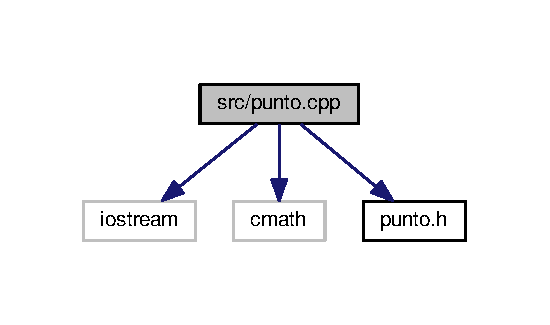
\includegraphics[width=264pt]{punto_8cpp__incl}
\end{center}
\end{figure}
\subsection*{Funciones}
\begin{DoxyCompactItemize}
\item 
double \hyperlink{punto_8cpp_a9c93fd6721d3b594dbbcfb77a92a2880}{distancia} (\hyperlink{classPunto}{Punto} p1, \hyperlink{classPunto}{Punto} p2)
\begin{DoxyCompactList}\small\item\em Funciones auxiliares (no son métodos de la clase) \end{DoxyCompactList}\item 
\hyperlink{classPunto}{Punto} \hyperlink{punto_8cpp_a119f914f219e98be4c2c93b5138e97da}{punto\+Medio} (\hyperlink{classPunto}{Punto} p1, \hyperlink{classPunto}{Punto} p2)
\begin{DoxyCompactList}\small\item\em Calcula el punto que está entre dos puntos dados con distancia mínima a ambos. \end{DoxyCompactList}\end{DoxyCompactItemize}


\subsection{Descripción detallada}
Implementación de la clase {\ttfamily \hyperlink{classPunto}{Punto}}. 

\begin{DoxyAuthor}{Autor}
M\+P-\/\+D\+G\+IM -\/ Grupo A 
\end{DoxyAuthor}


\subsection{Documentación de las funciones}
\index{punto.\+cpp@{punto.\+cpp}!distancia@{distancia}}
\index{distancia@{distancia}!punto.\+cpp@{punto.\+cpp}}
\subsubsection[{\texorpdfstring{distancia(\+Punto p1, Punto p2)}{distancia(Punto p1, Punto p2)}}]{\setlength{\rightskip}{0pt plus 5cm}double distancia (
\begin{DoxyParamCaption}
\item[{{\bf Punto}}]{p1, }
\item[{{\bf Punto}}]{p2}
\end{DoxyParamCaption}
)}\hypertarget{punto_8cpp_a9c93fd6721d3b594dbbcfb77a92a2880}{}\label{punto_8cpp_a9c93fd6721d3b594dbbcfb77a92a2880}


Funciones auxiliares (no son métodos de la clase) 

Calcula la distancia entre dos puntos 
\begin{DoxyParams}{Parámetros}
{\em p1} & primer punto \\
\hline
{\em p2} & segundo punto \\
\hline
\end{DoxyParams}
\begin{DoxyReturn}{Devuelve}
la distancia entre el punto {\itshape p1} y el punto {\itshape p2} 
\end{DoxyReturn}


Definición en la línea 40 del archivo punto.\+cpp.


\begin{DoxyCode}
40                                     \{
41     \textcolor{keywordflow}{return} sqrt((p1.\hyperlink{classPunto_aa218292fec9bad5ec6d71d4bd9173d9d}{getX}()-p2.\hyperlink{classPunto_aa218292fec9bad5ec6d71d4bd9173d9d}{getX}())*(p1.\hyperlink{classPunto_aa218292fec9bad5ec6d71d4bd9173d9d}{getX}()-p2.\hyperlink{classPunto_aa218292fec9bad5ec6d71d4bd9173d9d}{getX}()) +
42          (p1.\hyperlink{classPunto_a214978b8bbae48ca5927f2e56fb3bd22}{getY}()-p2.\hyperlink{classPunto_a214978b8bbae48ca5927f2e56fb3bd22}{getY}())*(p1.\hyperlink{classPunto_a214978b8bbae48ca5927f2e56fb3bd22}{getY}()-p2.\hyperlink{classPunto_a214978b8bbae48ca5927f2e56fb3bd22}{getY}()));
43 \}
\end{DoxyCode}


Gráfico de llamadas para esta función\+:
\nopagebreak
\begin{figure}[H]
\begin{center}
\leavevmode
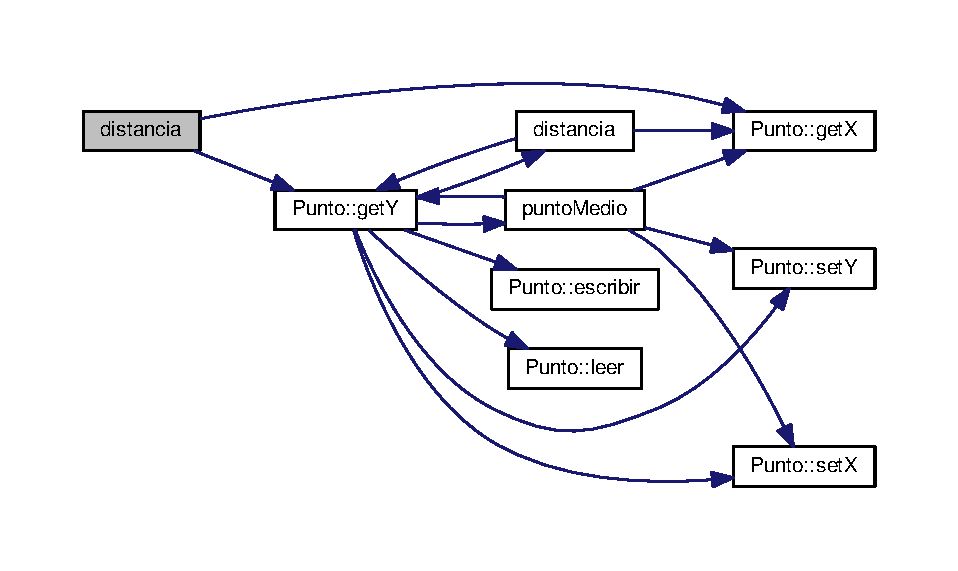
\includegraphics[width=350pt]{punto_8cpp_a9c93fd6721d3b594dbbcfb77a92a2880_cgraph}
\end{center}
\end{figure}


\index{punto.\+cpp@{punto.\+cpp}!punto\+Medio@{punto\+Medio}}
\index{punto\+Medio@{punto\+Medio}!punto.\+cpp@{punto.\+cpp}}
\subsubsection[{\texorpdfstring{punto\+Medio(\+Punto p1, Punto p2)}{puntoMedio(Punto p1, Punto p2)}}]{\setlength{\rightskip}{0pt plus 5cm}{\bf Punto} punto\+Medio (
\begin{DoxyParamCaption}
\item[{{\bf Punto}}]{p1, }
\item[{{\bf Punto}}]{p2}
\end{DoxyParamCaption}
)}\hypertarget{punto_8cpp_a119f914f219e98be4c2c93b5138e97da}{}\label{punto_8cpp_a119f914f219e98be4c2c93b5138e97da}


Calcula el punto que está entre dos puntos dados con distancia mínima a ambos. 


\begin{DoxyParams}{Parámetros}
{\em p1} & primer punto \\
\hline
{\em p2} & segundo punto \\
\hline
\end{DoxyParams}
\begin{DoxyReturn}{Devuelve}
un punto entre el punto {\itshape p1} y el punto {\itshape p2} con distancia mínima a ambos 
\end{DoxyReturn}


Definición en la línea 53 del archivo punto.\+cpp.


\begin{DoxyCode}
53                                     \{
54     \hyperlink{classPunto}{Punto} pMedio;
55     pMedio.\hyperlink{classPunto_a51ae6616f828bb2b4111bc8ace49dbca}{setX}((p1.\hyperlink{classPunto_aa218292fec9bad5ec6d71d4bd9173d9d}{getX}()+p2.\hyperlink{classPunto_aa218292fec9bad5ec6d71d4bd9173d9d}{getX}())/2.0);
56     pMedio.\hyperlink{classPunto_a6a0f8adb5946f31a7867a06f54d97462}{setY}((p1.\hyperlink{classPunto_a214978b8bbae48ca5927f2e56fb3bd22}{getY}()+p2.\hyperlink{classPunto_a214978b8bbae48ca5927f2e56fb3bd22}{getY}())/2.0);
57     \textcolor{keywordflow}{return} pMedio;
58 \}
\end{DoxyCode}


Gráfico de llamadas para esta función\+:
\nopagebreak
\begin{figure}[H]
\begin{center}
\leavevmode
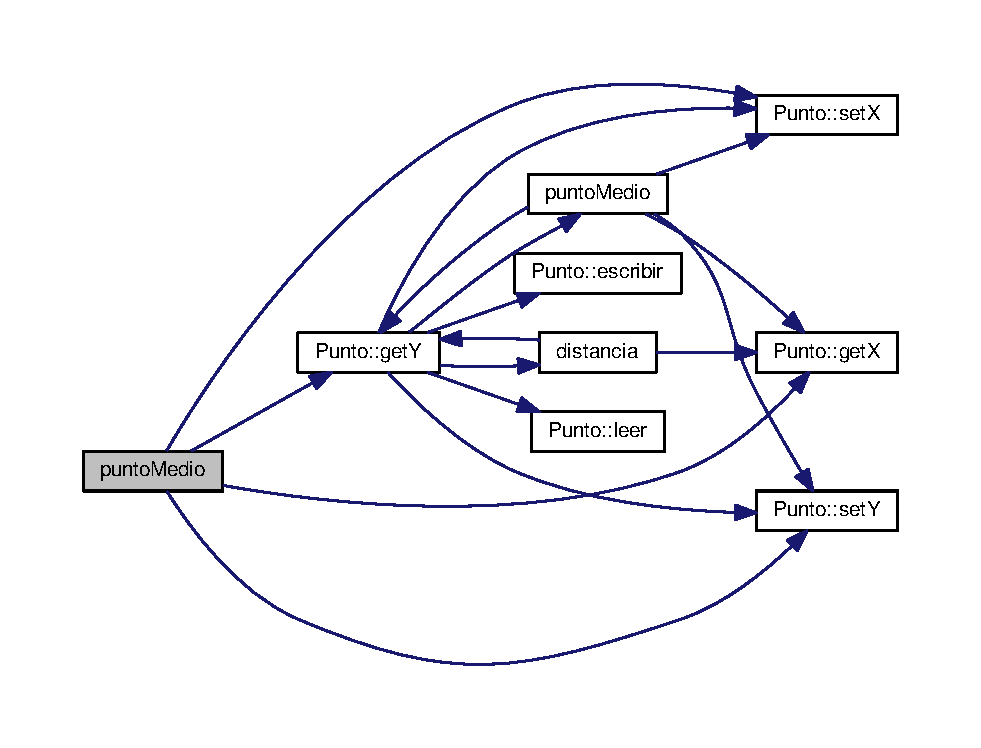
\includegraphics[width=350pt]{punto_8cpp_a119f914f219e98be4c2c93b5138e97da_cgraph}
\end{center}
\end{figure}



%--- End generated contents ---

% Index
\backmatter
\newpage
\phantomsection
\clearemptydoublepage
\addcontentsline{toc}{chapter}{Índice}
\printindex

\end{document}
